\documentclass[10pt,a4paper]{article}
\usepackage[utf8]{inputenc}
\usepackage[spanish]{babel}
\usepackage{geometry}
\geometry{top=1.5cm, bottom=1.5cm, left=1.5cm, right=1.5cm}
\usepackage{booktabs}
\usepackage{tabularx}
\usepackage{enumitem}
\usepackage{cite}
\usepackage{amsmath}
\usepackage{graphicx} 

\title{
    \vspace{-1.5cm}
    \small \textbf{UNIVERSIDAD TÉCNICA ESTATAL DE QUEVEDO} \\
    Carrera de Ingeniería de Software --- Aplicaciones Distribuidas (ISR-701) \\
    \large \vspace{0.3cm} \textbf{ANÁLISIS DE CASO: Fallo en Sistema Distribuido Real} \\
    \small \textit{Caso: Amazon Web Services --- Fallo de us-east-1 (Abril 2011)}
}
\author{
    \textbf{Grupo:} EQUIPO D \\
    \textbf{Integrantes:} ALVAREZ PARRAGA JEREMY ALEXIS \\
    AUCATOMA CELORIO JHINSON STALYN \\
    CARPIO MENDOZA CARLOS JOSE
}
\date{Semana 3 | Unidad 1 | 18-24 Mayo 2026}

\begin{document}

\maketitle

\section{Descripción del Incidente y Línea de Tiempo}
El 21 de abril de 2011 a las 00:47 UTC, la región us-east-1 de AWS sufrió una degradación crítica en los servicios Amazon EC2 y RDS durante 96 horas, alcanzando la recuperación el 24 de abril \cite{aws2011}. Un error operativo manual en un cambio de configuración de red desvió el tráfico de replicación troncal hacia una red secundaria de alta latencia. 

Esto provocó que miles de instancias de Amazon Elastic Block Store (EBS) dejaran de sincronizarse correctamente e iniciaran simultáneamente un proceso automático de re-replicación (\textit{re-mirroring}). Esto desató una \textbf{\textit{re-mirroring storm}} (tormenta de re-espejado): la demanda masiva saturó el almacenamiento de la zona de disponibilidad (AZ) afectada, provocando que más servidores quedaran sin respaldo y bloqueando los volúmenes en un estado inaccesible (\textit{stuck}).

\begin{table}[h!]
\footnotesize
\centering
\caption{Cronología del fallo en us-east-1}
\vspace{0.1cm}
\begin{tabularx}{\textwidth}{lX}
\toprule
\textbf{Hora (UTC)} & \textbf{Evento / Estado del Sistema} \\
\midrule
\textbf{21 Apr 00:47} & Error de configuración manual: tráfico troncal desviado a red de alta latencia. \\
\textbf{21 Apr 00:47 - 01:30} & Fallo de sincronización y detección masiva de pérdida de réplicas EBS. Inicio de la tormenta. \\
\textbf{21 Apr $\sim$01:30} & Saturación del almacenamiento en la AZ. Las instancias EC2 entran en estado bloqueado (\textit{stuck}). \\
\textbf{21 Apr 08:00} & AWS publica la primera declaración oficial en el Service Health Dashboard. \\
\textbf{24 Apr $\sim$08:00} & Estabilización integral del servicio y publicación del informe \textit{post-mortem} oficial. \\
\bottomrule
\end{tabularx}
\end{table}

\section{Identificación de Causas Raíz (Diagrama de Ishikawa)}
El desglose analítico de los factores determinantes del colapso se modela a continuación mediante el Diagrama de Ishikawa adjuntado por el equipo, distribuyendo las vulnerabilidades operativas, de entorno y de software:

\begin{figure}[h!]
\centering
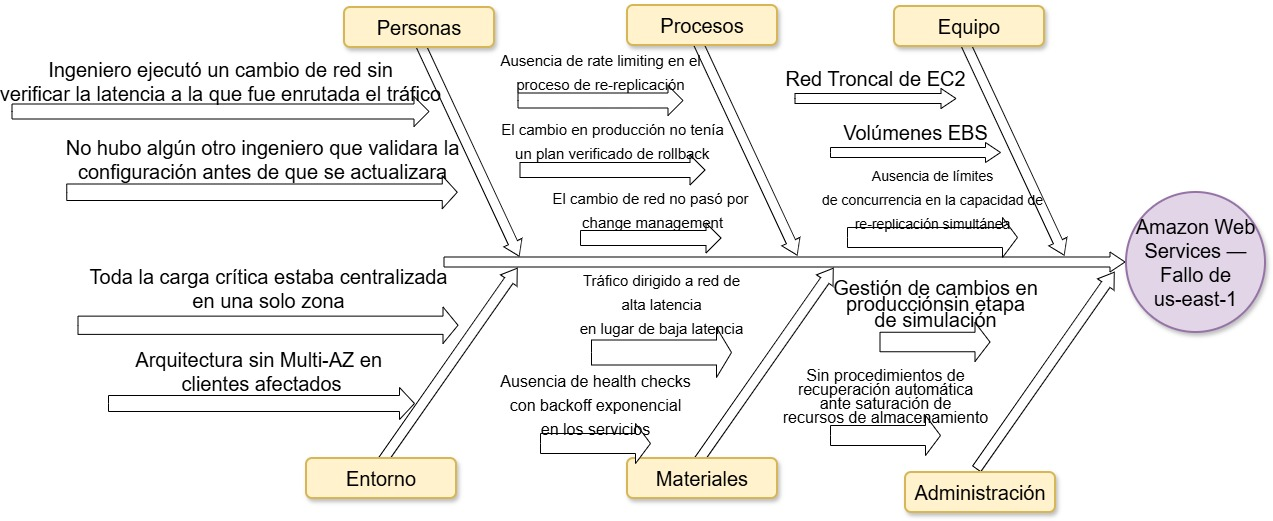
\includegraphics[width=0.92\textwidth]{ishikawa.jpeg} 
\caption{Diagrama de Ishikawa del incidente de AWS (2011).}
\end{figure}

\section{Impacto Cuantificado y Acciones de Mitigación}

\textbf{Impacto del Incidente:}
El fallo afectó a plataformas que dependían de los servicios de AWS, entre ellas Heroku, Reddit, Foursquare y Quora. Aproximadamente el $1.87\%$ de las instancias EC2 de la región us-east-1 quedaron inaccesibles de forma permanente. La interrupción tuvo una duración cercana a las $\sim$96 horas, ocasionando pérdidas económicas debido a la caída de servicios que dependían de una sola zona de disponibilidad.

\textbf{Estrategias de Mitigación y Acciones Post-Incidente:}
Como se detalla en el reporte oficial \cite{aws2011}, AWS aplicó varias medidas para intentar estabilizar y recuperar el sistema afectado:

\begin{itemize}[noitemsep, leftmargin=*]
    \item \textbf{Recuperación Progresiva:} La empresa restauró gradualmente las instancias EBS afectadas, recuperándolas una por una. Sin embargo, debido a la gravedad del incidente, alrededor del $13\%$ de los datos afectados no pudo recuperarse.

    \item \textbf{Comunicación y Transparencia:} AWS publicó su primer comunicado oficial el 21 de abril a las 08:00 UTC mediante el Service Health Dashboard, informando sobre el problema y manteniendo actualizaciones constantes hasta la publicación final del informe \textit{post-mortem} oficial.
\end{itemize}

\section{Lecciones Aprendidas y Aplicación al Proyecto Fin de Curso (PFC)}
\begin{enumerate}[leftmargin=*, noitemsep]
    \item \textbf{Modelo de Consistencia en el ADR:} El fallo demostró que un esquema de consistencia estricta ante particiones (Sistema CP según CAP \cite{brewer2000}) reduce la disponibilidad a cero ($A=0$). Documentaremos formalmente la postura de nuestro PFC en el ADR.
    \item \textbf{Patrón Circuit Breaker inter-servicios:} Para prevenir fallos en cascada equivalentes a la tormenta de EBS, añadiremos cortocircuitos técnicos (\textit{Circuit Breakers}) en los microservicios, evitando tormentas de reintentos concurrentes.
    \item \textbf{Inyección de Fallos Activas (Chaos Engineering):} Programaremos pruebas destructivas controladas en la entrega final de la Semana 17 (deteniendo contenedores Docker en caliente) para validar de forma real la autonomía de nuestros \textit{health checks}.
\end{enumerate}

\section{Conclusiones}

El fallo de AWS en 2011 demuestra la importancia de una buena planificación y monitoreo en los sistemas distribuidos. Aunque la redundancia ayuda a mejorar la disponibilidad de los servicios, este caso evidencia que no es suficiente si los mecanismos de recuperación no están correctamente controlados.

Además, este incidente permite comprender cómo un pequeño error de configuración puede generar fallos en cadena que afectan a millones de usuarios y servicios. También se resalta la necesidad de aplicar estrategias de tolerancia a fallos, monitoreo constante y planes de recuperación para reducir el impacto de este tipo de problemas en sistemas distribuidos\cite{tanenbaum2025}.

\begin{thebibliography}{9}
\small
\bibitem{aws2011} Amazon Web Services, ``Summary of the Amazon EC2 and Amazon RDS Service Disruption in the US East Region,'' \textit{AWS Service Health Dashboard}, Apr. 2011. [Online]. Available: https://aws.amazon.com/message/65648/
\bibitem{brewer2000} E. Brewer, ``Towards robust distributed systems,'' in \textit{Proc. 19th ACM Symp. Principles of Distributed Computing (PODC)}, 2000, p. 7.
\bibitem{tanenbaum2025} M. van Steen and A. S. Tanenbaum, \textit{Distributed Systems}, 4th ed., ver. 4.03. Maastricht, The Netherlands: Maarten van Steen, Jan. 2025.
\end{thebibliography}

\end{document}